\chapter{Processus global : de la compréhension des données à l’évaluation des modèles}
\newpage
\section{Introduction}
Ce chapitre est dédié à la modélisation des solutions d’intelligence artificielle intégrées dans l’application \textbf{MindCare-AI}. Il détaille le processus complet, depuis la compréhension et la préparation du dataset PPG+Dalia jusqu’à l’évaluation des modèles de classification de la fréquence cardiaque, en passant par le prétraitement des données, l’extraction de caractéristiques pertinentes, le choix des architectures adaptées, l’entraînement et l’analyse des performances.
Parallèlement, ce chapitre présente également la conception et l’intégration d’un chatbot intelligent, capable d’interagir avec les utilisateurs, de fournir des conseils personnalisés et d’exploiter les résultats des analyses physiologiques pour un accompagnement en temps réel.
L’utilisation de modèles avancés, de pipelines de prétraitement éprouvés et de techniques d’IA conversationnelle permet ainsi d’assurer à la fois une détection fiable des états physiologiques et une expérience utilisateur interactive, personnalisée et sécurisée.
\section{Collection et préparation des données}

Nous  commencons par la collection du dataset :

\subsection{Collection du jeu de données}

La première étape du processus a consisté à collecter et explorer le jeu de données adapté aux objectifs de l’application MindCare-AI. Cette phase, essentielle dans la démarche CRISP-DM, vise à comprendre la nature des données disponibles, à identifier les caractéristiques pertinentes pour l’analyse des signaux physiologiques, et à anticiper les éventuels problèmes de qualité ou de représentativité. Un soin particulier a été apporté à la sélection d’un dataset répondant aux critères de diversité, de fiabilité et de richesse des informations, afin de garantir la robustesse des modèles développés.

\subsubsection{Choix du jeu de données}


Pour ce projet, le choix s’est porté sur le PPG+Dalia dataset, un benchmark reconnu pour l’analyse des signaux (PPG) et l’estimation de la fréquence cardiaque dans des conditions réelles. Ce jeu de données comprend les enregistrements de 15 sujets, réalisés lors d’activités variées, avec des capteurs portés au poignet (PPG) et une référence ECG thoracique. Il offre ainsi une base solide pour le développement de modèles de classification robustes et pour l’intégration d’un chatbot capable d’exploiter ces analyses dans un contexte d’accompagnement personnalisé.
\subsubsection{Description des jeux de données}
\subsubsection{PPG+Dalia}
Le premier jeu de données, \textbf{PPG+Dalia}, contient des signaux physiologiques enregistrés auprès de 15 participants lors d'activités variées (marche, repos, travail, etc.). Chaque enregistrement comprend :
\begin{itemize}
    \item Des signaux PPG issus de capteurs portés au poignet,
    \item Des signaux ECG de référence,
    \item Des labels de fréquence cardiaque (HR) extraits de l’ECG,
    \item Parfois d’autres signaux physiologiques (EDA, température).
\end{itemize}
Ce dataset permet d’étudier la variabilité de la fréquence cardiaque dans des conditions réelles et de développer des modèles de classification robustes.

\begin{table}[H]
    \centering
    \caption{Caractéristiques démographiques des sujets du dataset PPG+Dalia}
    \begin{tabular}{cccccccc}
        \hline
        \textbf{Subject ID} & \textbf{Gender} & \textbf{Age [years]} & \textbf{Height [cm]} & \textbf{Weight [kg]} & \textbf{Skin Type} & \textbf{Fitness} \\
        \hline
        S1  & m & 34 & 182 & 78  & 3 & 6 \\
        S2  & m & 28 & 189 & 80  & 3 & 5 \\
        S3  & m & 25 & 170 & 60  & 3 & 5 \\
        S4  & m & 25 & 168 & 57  & 4 & 5 \\
        S5  & f & 21 & 180 & 70  & 3 & 4 \\
        S6  & f & 37 & 176 & 70  & 3 & 1 \\
        S7  & f & 21 & 168 & 58  & 3 & 2 \\
        S8  & m & 43 & 179 & 70  & 3 & 5 \\
        S9  & f & 28 & 167 & 60  & 4 & 5 \\
        S10 & f & 55 & 164 & 56  & 4 & 5 \\
        S11 & f & 24 & 168 & 62  & 3 & 5 \\
        S12 & m & 43 & 195 & 105 & 3 & 5 \\
        S13 & f & 21 & 170 & 63  & 3 & 6 \\
        S14 & f & 26 & 170 & 67  & 3 & 4 \\
        S15 & m & 28 & 183 & 79  & 2 & 5 \\
        \hline
        \multicolumn{2}{c}{\textbf{Moyenne $\pm$ écart-type}} & 30.60$\pm$9.59 & 175.27$\pm$8.78 & 69.00$\pm$12.35 & & \\
        \hline
    \end{tabular}
    \label{tab:ppg_dalia_subjects}
\end{table}

\subsubsection{Emotions dataset for NLP }

Ce jeu de données est une collection de phrases annotées selon différentes émotions, conçu pour les tâches de classification en traitement automatique du langage naturel (NLP). Il se compose de documents textuels, chacun associé à une étiquette d’émotion (par exemple : joie, tristesse, colère, peur, amour, surprise). Le dataset est organisé en trois sous-ensembles distincts : entraînement, validation et test, facilitant ainsi le développement, l’évaluation et la comparaison de modèles de classification d’émotions.

\textbf{Exemple d’entrée :}
\begin{quote}
\textit{i feel like I am still looking at a blank canvas blank pieces of paper ; sadness}
\end{quote}

Ce corpus est particulièrement utile pour entraîner des modèles capables de détecter automatiquement l’émotion exprimée dans un texte, ce qui peut s’avérer précieux pour l’analyse de commentaires clients, la modération de contenus ou encore l’accompagnement psychologique personnalisé via un chatbot.  
Le jeu de données a été préparé grâce aux contributions de la communauté et s’appuie sur des techniques de référence en NLP~\cite{Emotion_Data}.  
Il constitue une ressource précieuse pour la recherche et le développement de solutions d’intelligence artificielle centrées sur la compréhension des émotions humaines.
\subsection{Analyse de distribution}

Pour évaluer la représentativité et la diversité des jeux de données utilisés dans MindCare-AI, nous avons analysé la distribution de plusieurs variables clés.

\subsubsection{PPG+Dalia}

L’analyse de la distribution des caractéristiques démographiques et physiologiques des sujets du dataset PPG+Dalia révèle une diversité en termes d’âge, de sexe, de taille, de condition physique et de fréquence cardiaque.
La figure~\ref{fig:Dist_dashboard} présente un tableau de bord synthétique de la distribution des principales variables du dataset.
\begin{figure}[H]
    \centering
    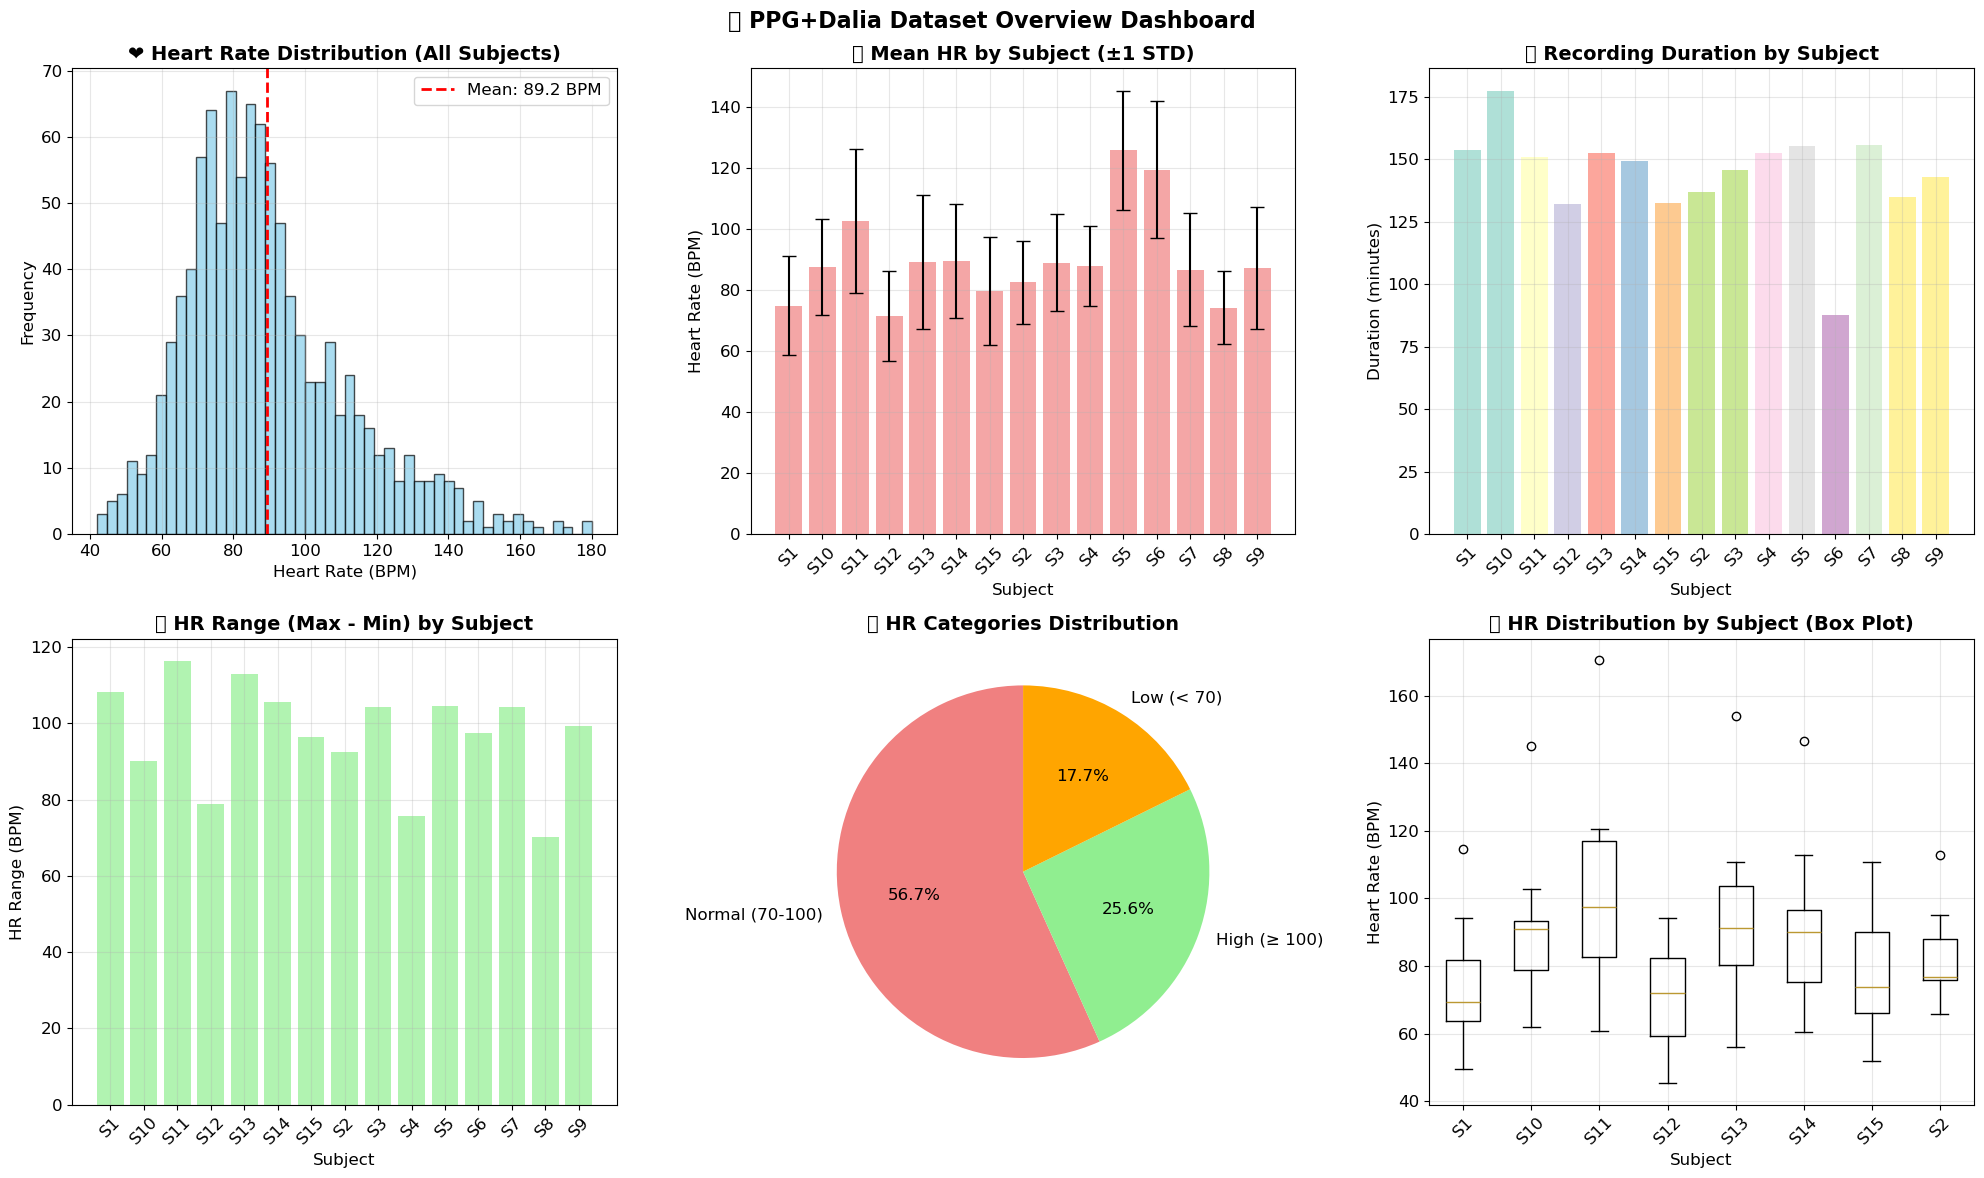
\includegraphics[width=1\textwidth]{Figures/Distribution PPG.png}
    \caption{Tableau de bord de la distribution des variables du dataset PPG+Dalia : fréquence cardiaque, durée d’enregistrement, catégories}
    \label{fig:Dist_dashboard}
\end{figure}



\subsubsection{Emotions dataset for NLP}

Pour le jeu de données Emotions, la distribution des différentes classes d’émotions est un facteur important pour l’équilibre de l’apprentissage. La figure~\ref{fig:dist_emotions_train} montre la répartition initiale des étiquettes d’émotions dans le corpus d’entraînement.

La distribution initiale est la suivante :
\begin{itemize}
    \item joy : 5362
    \item sadness : 4666
    \item anger : 2159
    \item fear : 1937
    \item love : 1304
    \item surprise : 572
\end{itemize}

\begin{figure}[H]
    \centering
    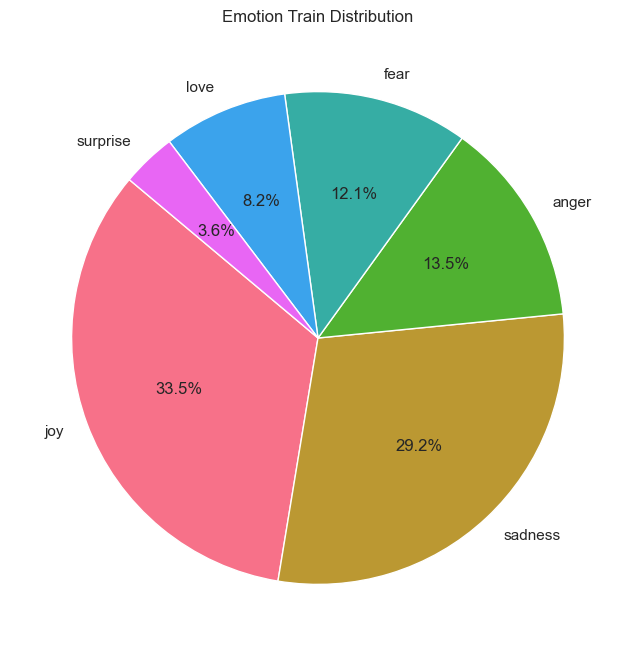
\includegraphics[width=0.6\textwidth]{Figures/emtion_train_distribution.png}
    \caption{Distribution initiale des classes d’émotions dans le dataset d’entraînement}
    \label{fig:dist_emotions_train}
\end{figure}

On constate un déséquilibre important entre les différentes classes. Pour garantir un apprentissage équitable du modèle, nous avons procédé à un équilibrage du dataset.

Cette analyse permet de vérifier l’absence de biais majeur et d’anticiper d’éventuels déséquilibres à corriger lors de l’entraînement des modèles.

\subsection{Préparation et prétraitement des données}

Le prétraitement des données est une étape clé pour garantir la qualité des analyses et la performance des modèles. Les étapes suivantes ont été réalisées pour chaque jeu de données, en s’appuyant sur des scripts Python dédiés.

\paragraph{Pour le dataset PPG+Dalia :}
\begin{itemize}
    \item \textbf{Chargement automatique et vérification des fichiers sujets} grâce à une classe dédiée (\texttt{PPGDaliaDataExplorer}), permettant de parcourir et d’importer tous les fichiers \texttt{.pkl} du dossier de données.
    \item \textbf{Extraction des signaux physiologiques} : récupération des signaux PPG (BVP), ECG, EDA, température, ainsi que des labels de fréquence cardiaque (HR) pour chaque sujet.
    \item \textbf{Synchronisation et nettoyage} : gestion des valeurs manquantes, conversion des clés binaires, suppression des signaux incomplets ou aberrants.
    \item \textbf{Analyse de structure et statistiques globales} : calcul automatique du nombre de sujets, de la durée totale, des types de signaux disponibles, de la distribution des valeurs de HR, etc.
    \item \textbf{Découpage en fenêtres temporelles} : segmentation des signaux bruts en fenêtres de taille fixe (par exemple 10 secondes, soit 640 échantillons à 64 Hz) pour l’extraction de caractéristiques locales.
    \item \textbf{Filtrage passe-bande} : application d’un filtre numérique (0.5–4 Hz) sur le signal PPG pour éliminer le bruit et les artefacts.
    \item \textbf{Extraction de caractéristiques avancées} : calcul de descripteurs temporels (moyenne, médiane, écart-type, etc.), fréquentiels (énergie spectrale, fréquence dominante, etc.), et ajout de variables démographiques synthétiques (âge, genre, fitness).
    \item \textbf{Construction des labels de classification} : attribution d’une classe (basse, normale, élevée) à chaque fenêtre selon la médiane du HR de référence.
    \item \textbf{Équilibrage intelligent des classes} : rééchantillonnage pour obtenir un nombre similaire de fenêtres par classe, avec sur-échantillonnage contrôlé si besoin.
\end{itemize}

\paragraph{Pour le dataset Emotions (NLP) :}
\begin{itemize}
    \item \textbf{Chargement des données} : Import des fichiers \texttt{train.csv}, \texttt{val.csv} et \texttt{test.csv} dans des DataFrames pandas.
    \item \textbf{Analyse et visualisation de la distribution des émotions} : Comptage des occurrences de chaque émotion et visualisation par diagramme circulaire pour détecter les déséquilibres.
    \item \textbf{Filtrage des classes minoritaires} : Suppression des émotions trop peu représentées (\textit{love}, \textit{surprise}) dans tous les ensembles pour garantir la robustesse du modèle.
    \item \textbf{Équilibrage du dataset d'entraînement} : Sous-échantillonnage ou sur-échantillonnage de chaque classe pour obtenir le même nombre d’exemples par émotion (par la méthode du tirage aléatoire avec ou sans remise).
    \item \textbf{Préparation des données textuelles et des labels} : Extraction des textes et des étiquettes d’émotion pour chaque ensemble (train, validation, test).
    \item \textbf{Encodage des labels} : Transformation des émotions en labels numériques à l’aide de \texttt{LabelEncoder}.
    \item \textbf{Tokenisation et vectorisation} : Création d’un \texttt{Tokenizer} Keras (vocabulaire limité à 10\,000 mots), conversion des textes en séquences d’indices, puis padding à une longueur fixe (50 tokens).
    \item \textbf{Conversion des labels en one-hot} : Transformation des labels numériques en vecteurs binaires pour l’apprentissage supervisé.
    \item \textbf{Vérification des dimensions finales} : Contrôle du vocabulaire, de la longueur des séquences et du nombre de classes pour garantir la cohérence des entrées du modèle.
\end{itemize}

\begin{center}
    
\includegraphics[height=1.4cm]{Figures/jupyter.png}\\
    \textit{Toutes ces étapes de préparation et de prétraitement ont été réalisées et automatisées dans un notebook \textbf{Jupyter}, assurant un pipeline reproductible et interactif.}
\end{center}

Ce pipeline de préparation garantit la qualité, la diversité et la pertinence des données utilisées pour l’entraînement et l’évaluation des modèles d’IA intégrés dans MindCare-AI.

\section{Modélisation et évaluation}

Cette section présente la démarche de modélisation des différents modules d’intelligence artificielle intégrés dans MindCare-AI, ainsi que l’évaluation expérimentale des performances obtenues. Deux axes principaux sont abordés : la classification de la fréquence cardiaque à partir des signaux physiologiques (PPG+Dalia) et la classification des émotions à partir de textes (dataset Emotions). Enfin, l’intégration de ces modèles dans le chatbot est discutée.

\subsection{Modélisation pour la classification de la fréquence cardiaque (PPG+Dalia)}

\paragraph{Choix des modèles et pipeline}
Pour la tâche de classification de la fréquence cardiaque, plusieurs modèles d’apprentissage automatique ont été testés, notamment : \textit{Random Forest}, \textit{Gradient Boosting}, \textit{SVM}, \textit{MLP}, et différentes variantes d’arbres de décision. Le pipeline inclut la normalisation des caractéristiques, la sélection de variables pertinentes et l’entraînement sur des fenêtres temporelles extraites du signal PPG.

\paragraph{Entraînement et validation croisée}
Les modèles ont été entraînés sur un jeu de données équilibré, avec une validation croisée pour évaluer la robustesse. Les métriques utilisées incluent la précision, le rappel, la F1-score et la matrice de confusion pour chaque classe (basse, normale, élevée).

\paragraph{Résultats}
Le meilleur modèle obtenu  Gradient Boosting  atteint une précision de \textbf{96,7\%} sur le jeu de test, avec une bonne capacité à distinguer les trois classes de fréquence cardiaque. Les résultats détaillés sont présentés dans le tableau~\ref{tab:hr_classification_results} et la figure~\ref{fig:hr_confusion_matrix}.

% Exemple de tableau de résultats
\begin{table}[H]
    \centering
    \caption{Performances des modèles de classification de la fréquence cardiaque}
    \begin{tabular}{lcccc}
        \hline
        \textbf{Modèle} & \textbf{Accuracy} & \textbf{F1-score} & \textbf{Overfit} \\
        \hline
        Gradient Boosting & 0.967 & 0.967 & 0.033 \\
        Decision Tree     & 0.683 & 0.689 & 0.183 \\
        Random Forest     & 0.867 & 0.867 & 0.112 \\
        XGBoost           & 0.933 & 0.933 & 0.067 \\
        SVM               & 0.8 & 0.81 & 0.112 \\
        \hline
    \end{tabular}
    \label{tab:hr_classification_results}
\end{table}

\begin{figure}[H]
    \centering
    \includegraphics[width=0.6\textwidth]{Figures/confusion matrix.png}
    \caption{Matrice de confusion Gradient Boosting HR}
    \label{fig:hr_confusion_matrix}
\end{figure}

\subsection{Modélisation pour la classification des émotions (NLP)}

\paragraph{Architecture du modèle}
Pour la classification des émotions, un modèle de deep learning basé sur un réseau de neurones convolutionnel (CNN) a été développé. Le pipeline comprend la tokenisation des textes, le padding, l’encodage des labels et l’entraînement du modèle sur le dataset équilibré.

\paragraph{Entraînement et évaluation}
Le modèle a été entraîné sur l’ensemble d’entraînement, avec validation sur un ensemble séparé. Les performances sont évaluées en termes d’accuracy, de F1-score et de matrice de confusion.

\paragraph{Résultats}
Le modèle atteint une précision de \textbf{94.24\%} sur le jeu de test, avec une bonne capacité à distinguer les principales émotions (joie, tristesse, colère, peur). Les résultats sont illustrés dans la figure~\ref{fig:emotion_confusion_matrix}.

\begin{figure}[H]
    \centering
    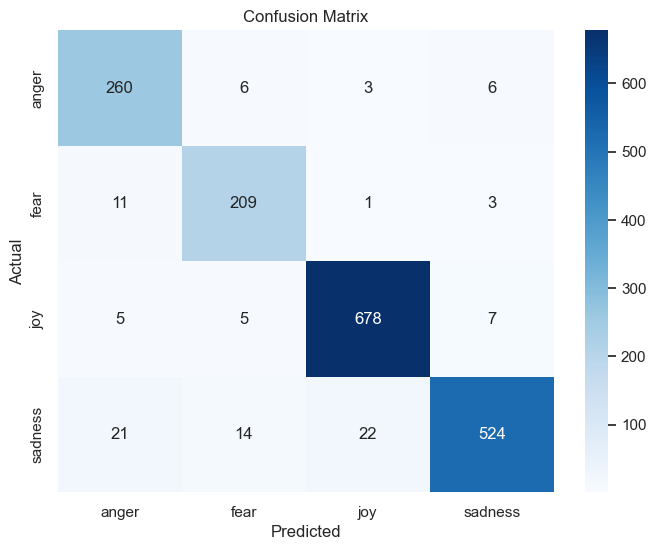
\includegraphics[width=0.6\textwidth]{Figures/matrice_emotion.png}
    \caption{Matrice de confusion du modèle de classification des émotions}
    \label{fig:emotion_confusion_matrix}
\end{figure}

\subsection{Intégration et évaluation dans le chatbot}

Les modèles de classification de la fréquence cardiaque et des émotions ont été intégrés au sein du chatbot MindCare-AI. L’évaluation de l’expérience utilisateur a montré que le système est capable de fournir des retours personnalisés, des conseils adaptés et d’améliorer le suivi du bien-être mental de manière interactive et sécurisée.

\paragraph{Limites et perspectives}
Parmi les principales limites identifiées figurent la taille relativement restreinte des jeux de données, la variabilité inter-individuelle des signaux physiologiques, ainsi que la nécessité d’une validation clinique plus approfondie. Les perspectives d’amélioration incluent l’augmentation du volume de données, l’intégration de signaux physiologiques supplémentaires et l’optimisation continue des modèles d’intelligence artificielle afin d’accroître la robustesse et la pertinence des recommandations fournies par le système.

